\chapter{Графики, преобразования и исследование функций}\label{chap:exam-functions}\markright{Глава 21}
\section{Область определения, нули и знаки}
Значение функции и значение аргумента играют разные роли: \(f(a)=b\) задаёт точку \((a;b)\), а не \((b;a)\). Для формулы с дробью исключают нули знаменателя, для корня чётной степени требуют неотрицательный подкоренной аргумент. У составной функции все условия действуют одновременно. Сокращение множителей упрощает значения, но не возвращает исключённые точки в исходную область определения.
\begin{definition}\term{Промежуток знакопостоянства} (\emph{interval of constant sign}) --- промежуток, на котором функция всюду положительна либо всюду отрицательна. \par\term{Множество уровня} (\emph{level set}) значения \(c\) --- множество всех \(x\), для которых \(f(x)=c\). На графике это пересечения с горизонтальной прямой \(y=c\).\end{definition}
\begin{example}Для \(f(x)=\frac{x^2-1}{x-1}\) область \(\mathbb R\setminus\{1\}\). При \(x\ne1\) значение равно \(x+1\). График --- прямая с выколотой точкой \((1;2)\). Область значений --- \(\mathbb R\setminus\{2\}\). Нуль \(-1\) допустим, а \(x=1\) нулём не является.\end{example}
\section{Преобразования графиков}
\begin{theorem}[Сдвиг и растяжение графика]
Пусть \(g(x)=a f(b(x-h))+k\), где \(a,b\ne0\). Точка \((u;v)\) графика \(f\) переходит в точку
\[
\left(h+\frac ub;\ k+av\right)
\]
графика \(g\). Смена знака \(a\) отражает график относительно прямой \(y=k\), а смена знака \(b\) --- относительно прямой \(x=h\).
\end{theorem}
\begin{proof}Подставим \(x=h+\frac{u}{b}\). Тогда \(b(x-h)=u\), \(g(x)=af(u)+k=av+k\). Обратно, каждый допустимый \(x\) имеет такое представление, поэтому получены все точки.\end{proof}
В частности, \(f(x-h)+k\) сдвигает график на \(h\) вправо и \(k\) вверх. Запись \(f(2x)\) сжимает горизонтальные расстояния вдвое; \(2f(x)\) растягивает вертикальные вдвое. Для \(|f(x)|\) отрицательную часть отражают вверх, положительную сохраняют. Для \(f(|x|)\) сохраняют правую часть и отражают её влево; части с отрицательным исходным аргументом не используются.
\begin{example}Построим \(y=-2|x-1|+3\). График \(|x|\) сдвигаем вправо на один, отражаем относительно горизонтальной оси, растягиваем вертикально вдвое и поднимаем на три. Вершина \((1;3)\), область значений \(( -\infty;3]\), нули \(-\frac{1}{2}\) и \(\frac{5}{2}\). Функция возрастает до вершины и убывает после неё.\end{example}
\par\addvspace{2pt}\begin{lrbox}{\CatFlowBox}\begin{minipage}[t]{\linewidth}
\setlength{\parskip}{2pt}\setlength{\columnsep}{4.5mm}\setlength{\intextsep}{0pt}
\begin{wrapfigure}[10]{r}{54mm}
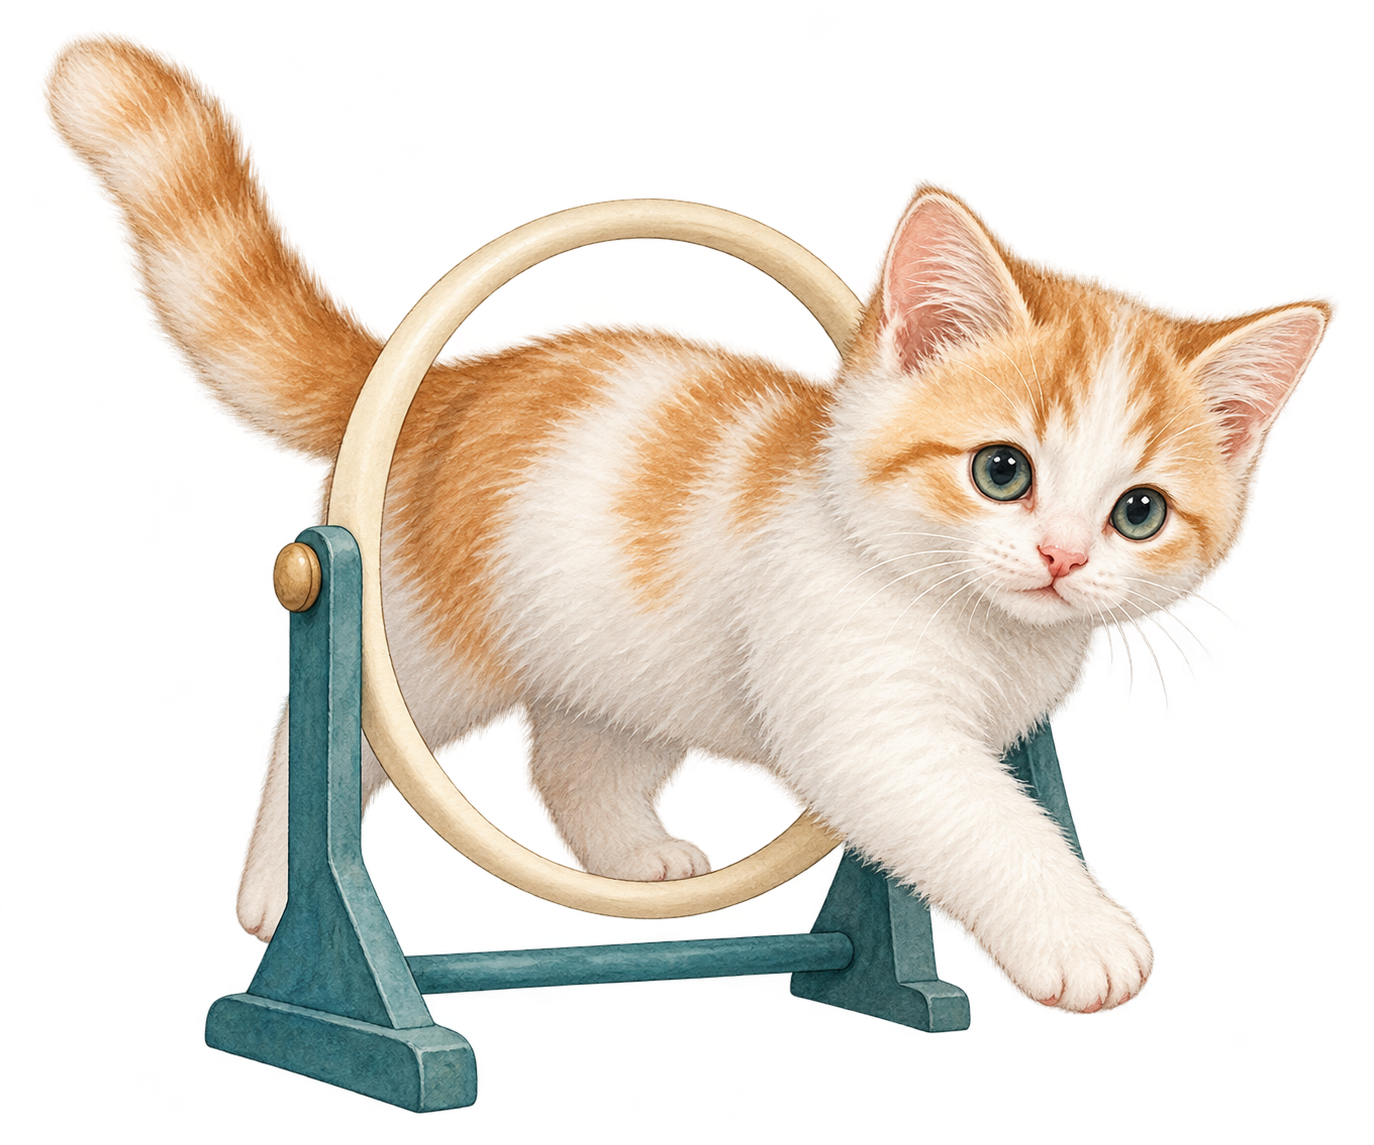
\includegraphics[width=54mm,height=58mm,keepaspectratio]{images/unique/art-212.png}
\label{catflow:212}
\end{wrapfigure}
При построении графика выбирают несколько опорных точек и преобразуют их по одной и той же формуле. Отдельно отмечают границы области определения, выколотые точки и точки соединения кусков. Если график содержит разрыв, нельзя соединять соседние нарисованные ветви через запрещённое значение аргумента. Для чётной функции достаточно построить половину графика и отразить её относительно вертикальной оси; для нечётной используется центральная симметрия относительно начала координат. Но сначала нужно проверить симметрию области определения: одной похожей формулы недостаточно. Такое построение позволяет получить качественно правильный рисунок без длинной таблицы значений и увидеть, какие ответы действительно достигаются.
\par\WFclear\end{minipage}\end{lrbox}%
\ifdim\dimexpr\ht\CatFlowBox+\dp\CatFlowBox\relax<58mm\dp\CatFlowBox=\dimexpr58mm-\ht\CatFlowBox\relax\fi%
\noindent\usebox{\CatFlowBox}\par\addvspace{2pt}
\begin{center}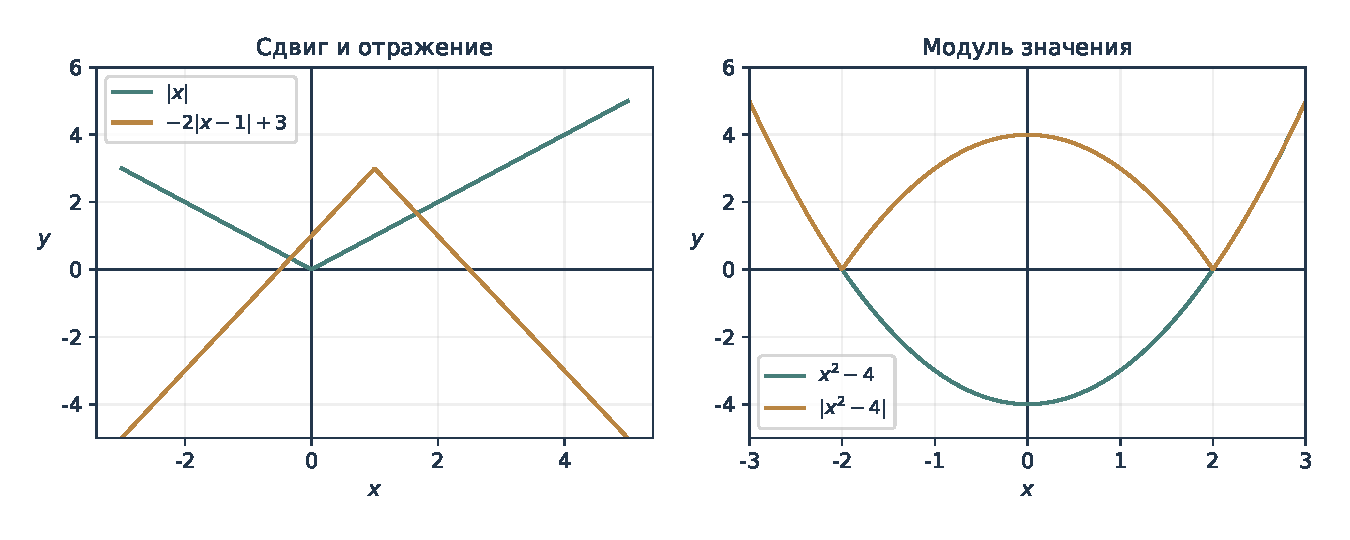
\includegraphics[width=\linewidth,height=74mm,keepaspectratio]{images/exam-functions-transform.pdf}\end{center}
\section{Квадратичная и дробно-линейная функции}
\begin{theorem}[Вершина параболы]
Для \(a\ne0\)
\[
ax^2+bx+c=a\left(x+\frac b{2a}\right)^2-\frac{b^2-4ac}{4a}.
\]
Вершина имеет абсциссу \(-\frac b{2a}\); при \(a>0\) она даёт минимум, при \(a<0\) --- максимум на всей прямой.
\end{theorem}
\par\addvspace{2pt}\begin{lrbox}{\CatFlowBox}\begin{minipage}[t]{\linewidth}
\setlength{\parskip}{2pt}\setlength{\columnsep}{4.5mm}\setlength{\intextsep}{0pt}
\begin{wrapfigure}[11]{l}{54mm}

\includegraphics[width=54mm,height=58mm,keepaspectratio]{images/unique/art-215.png}
\label{catflow:215}
\end{wrapfigure}
\textit{Доказательство.} Раскрытие квадрата даёт исходное выражение. Квадрат неотрицателен и равен нулю только в вершине; знак \(a\) задаёт направление неравенства.\hfill\(\blacksquare\)
\par\WFclear\end{minipage}\end{lrbox}%
\ifdim\dimexpr\ht\CatFlowBox+\dp\CatFlowBox\relax<58mm\dp\CatFlowBox=\dimexpr58mm-\ht\CatFlowBox\relax\fi%
\noindent\usebox{\CatFlowBox}\par\addvspace{2pt}

\begin{example}Для \(f(x)=x^2-4x+7=(x-2)^2+3\) на \([0;5]\) минимум равен \(3\) при \(x=2\). Максимум сравниваем на концах: \(f(0)=7\), \(f(5)=12\), поэтому он равен \(12\). Вершина параболы не обязана принадлежать заданному отрезку; тогда проверяют расположение отрезка относительно вершины.\end{example}
Для дробно-линейной функции при \(c\ne0\)
\[
\frac{ax+b}{cx+d}=\frac ac+\frac{bc-ad}{c^2}\frac1{x+\frac{d}{c}}.
\]
Если \(ad-bc\ne0\), это сдвинутая и растянутая гипербола с исключённым \(x=-\frac{d}{c}\). При \(ad-bc=0\) получается постоянное значение \(\frac{a}{c}\) с исключённой точкой, а не гипербола. Если \(c=0\), отдельно рассматривают линейную или постоянную функцию при \(d\ne0\).
\section{Кусочные функции и графический метод}
\begin{definition}\term{Кусочно заданная функция} (\emph{piecewise-defined function}) описывается разными формулами на указанных частях области определения. Если части пересекаются, значения формул в пересечении должны совпадать.\end{definition}
\begin{example}Пусть \(f(x)=x+2\) при \(x<0\) и \(f(x)=x^2\) при \(x\ge0\). В точке \(0\) ставим закрашенную точку \((0;0)\), а \((0;2)\) на прямой выколота. Уравнение \(f(x)=1\) даёт \(x=-1\) из первой части и \(x=1\) из второй; корень \(-1\) квадратного уравнения не добавляют повторно из второй части, поскольку там требуется \(x\ge0\).\end{example}
\par\addvspace{2pt}\begin{lrbox}{\CatFlowBox}\begin{minipage}[t]{\linewidth}
\setlength{\parskip}{2pt}\setlength{\columnsep}{4.5mm}\setlength{\intextsep}{0pt}
\begin{wrapfigure}[11]{l}{54mm}

\includegraphics[width=54mm,height=58mm,keepaspectratio]{images/unique/art-213.png}
\label{catflow:213}
\end{wrapfigure}
Пересечение графиков \(y=f(x)\) и \(y=g(x)\) решает уравнение \(f(x)=g(x)\) с общей областью определения. График помогает предположить число корней, но точное доказательство требует анализа формул, монотонности или другого установленного свойства. При чтении готового графика проверяй шкалу осей: один шаг сетки не обязан означать единицу. Если спрашивают число решений, считают различные аргументы пересечений, а не отдельные способы записи одного корня. Для неравенства \(f(x)>g(x)\) выбирают промежутки, где первый график выше второго, и исключают точки равенства и запрещённые аргументы. Вертикальная прямая может пересекать график функции не более чем в одной точке.
\par\WFclear\end{minipage}\end{lrbox}%
\ifdim\dimexpr\ht\CatFlowBox+\dp\CatFlowBox\relax<58mm\dp\CatFlowBox=\dimexpr58mm-\ht\CatFlowBox\relax\fi%
\noindent\usebox{\CatFlowBox}\par\addvspace{2pt}
\section{Монотонность, экстремумы и ограниченность}
\begin{definition}\term{Строго возрастающая функция} (\emph{strictly increasing function}) на множестве \(I\) удовлетворяет \(f(x_1)<f(x_2)\) при \(x_1<x_2\), \(x_1,x_2\in I\). \par Для \term{неубывающей функции} (\emph{nondecreasing function}) знак заменяется на \(\le\). \par\term{Строго убывающая функция} (\emph{strictly decreasing function}) удовлетворяет \(f(x_1)>f(x_2)\) при \(x_1<x_2\). \par\term{Невозрастающая функция} (\emph{nonincreasing function}) удовлетворяет \(f(x_1)\geq f(x_2)\) при \(x_1<x_2\). В обоих случаях аргументы принадлежат рассматриваемому множеству.\end{definition}
\begin{definition}\term{Локальный максимум} (\emph{local maximum}) во внутренней точке --- значение, не меньшее всех достаточно близких значений функции; локальный минимум определяется аналогично. \par\term{Наибольшее значение} (\emph{global maximum}) на множестве не меньше всех его значений и обязательно достигается. \par\term{Ограниченная функция} (\emph{bounded function}) имеет \(|f(x)|\le M\) на рассматриваемом множестве для некоторого \(M\).\end{definition}
У \(f(x)=x\) на \((0;1)\) нет наибольшего значения, хотя \(1\) --- точная верхняя грань. У \(\frac{1}{x}\) функция убывает на каждом из промежутков \(( -\infty;0)\), \((0;+\infty)\), но не на их объединении: например, \(-1<1\), а \(f(-1)<f(1)\). Промежутки, разделённые запрещённой точкой, нельзя автоматически объединять в один промежуток монотонности.
\section{Асимптоты и типы разрыва}
\begin{definition}\term{Вертикальная асимптота} (\emph{vertical asymptote}) \(x=a\) имеет место, если хотя бы один односторонний предел функции при \(x\to a\) бесконечен. \par\term{Наклонная асимптота} (\emph{oblique asymptote}) \(y=kx+b\) при \(x\to+\infty\) означает \(f(x)-(kx+b)\to0\). При \(k=0\) говорят о \term{горизонтальной асимптоте} (\emph{horizontal asymptote}). Условие при \(-\infty\) проверяют отдельно.\end{definition}
Пределы подробно определены в главе \ref{chap:c19}. Здесь асимптота означает неограниченное приближение по соответствующему условию; она может пересекаться с графиком. Для наклонной асимптоты, если соответствующие конечные пределы существуют, \(k=\lim \frac{f(x)}x\), \(b=\lim(f(x)-kx)\).
\begin{example}Деление даёт \(\frac{x^2+1}{x-1}=x+1+\frac2{x-1}\). Поэтому \(x=1\) --- вертикальная асимптота, \(y=x+1\) --- наклонная при обоих направлениях бесконечности. Для \(\frac{x^2-1}{x-1}\) при \(x\ne1\) асимптоты \(x=1\) нет: предел \(2\) конечен, точку можно доопределить.\end{example}
\begin{definition}\term{Устранимый разрыв} (\emph{removable discontinuity}) допускает конечный общий предел, но значение отсутствует либо отличается от предела. \par\term{Разрыв скачком} (\emph{jump discontinuity}) имеет два конечных различных односторонних предела. Бесконечное поведение даёт разрыв иного типа.\end{definition}
\begin{center}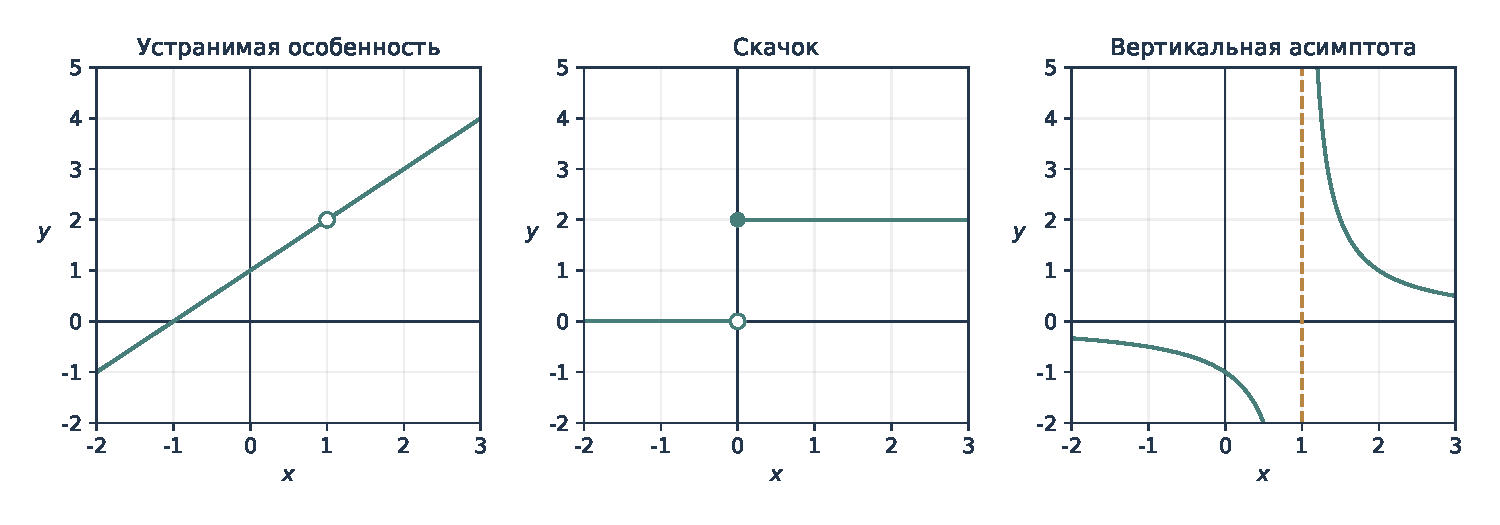
\includegraphics[width=\linewidth,height=68mm,keepaspectratio]{images/exam-functions-breaks.pdf}\end{center}
\par\addvspace{2pt}\begin{lrbox}{\CatFlowBox}\begin{minipage}[t]{\linewidth}
\setlength{\parskip}{2pt}\setlength{\columnsep}{4.5mm}\setlength{\intextsep}{0pt}
\begin{wrapfigure}[11]{r}{54mm}

\includegraphics[width=54mm,height=58mm,keepaspectratio]{images/unique/art-214.png}
\label{catflow:214}
\end{wrapfigure}
Исследование функции объединяет несколько проверок. Сначала устанавливают область определения, затем симметрию, нули, знаки и характерные точки. После этого изучают монотонность, экстремумы и поведение у границ области. Качественный эскиз обязан согласовываться со всеми этими данными: если формула положительна на промежутке, ветвь не должна случайно оказаться ниже оси. Для разрывной функции отдельно рассматривают каждый участок области определения и его односторонние границы. Когда появится производная, она упростит исследование монотонности, но не отменит проверки области и концов отрезка. Перед сдачей решения проверь, спрашивают ли аргумент точки экстремума или само значение функции: это разные числа.
\par\WFclear\end{minipage}\end{lrbox}%
\ifdim\dimexpr\ht\CatFlowBox+\dp\CatFlowBox\relax<58mm\dp\CatFlowBox=\dimexpr58mm-\ht\CatFlowBox\relax\fi%
\noindent\usebox{\CatFlowBox}\par\addvspace{2pt}
\relax

\par\addvspace{2pt}\begin{lrbox}{\CatFlowBox}\begin{minipage}[t]{\linewidth}
\setlength{\parskip}{2pt}\setlength{\columnsep}{4.5mm}\setlength{\intextsep}{0pt}
\begin{wrapfigure}[12]{r}{54mm}

\includegraphics[width=54mm,height=58mm,keepaspectratio]{images/unique/art-268.png}
\label{catflow:268}
\end{wrapfigure}
В обратной графической задаче неизвестна формула, а рисунок задаёт её ограничения. Координаты отмеченных точек читают по сетке, после чего составляют равенства для коэффициентов выбранного семейства функций. Одной точки недостаточно, если свободных коэффициентов несколько. Вершина параболы заменяет сразу две характеристики её положения; точка вне вершины определяет масштаб. Для пересечения двух графиков сначала восстанавливают обе формулы, затем решают полученное уравнение и проверяют корни. Видимый фрагмент рисунка не ограничивает область определения функции: второе пересечение может находиться за рамкой. Ответ зависит от данных точек и типа функции, а не от зрительной оценки толщины линии.
\par\WFclear\end{minipage}\end{lrbox}%
\ifdim\dimexpr\ht\CatFlowBox+\dp\CatFlowBox\relax<60mm\dp\CatFlowBox=\dimexpr60mm-\ht\CatFlowBox\relax\fi%
\noindent\usebox{\CatFlowBox}\par\addvspace{2pt}
\relax
\section{От рисунка к формуле}
Обратная графическая задача начинается с распознавания семейства функций. У квадратичной функции вершина \((h,k)\) даёт запись \(f(x)=a(x-h)^2+k\), но не определяет \(a\). Его находят по ещё одной точке, отличной от вершины. Если известны три точки с разными абсциссами, можно составить три линейных уравнения на \(a,b,c\) в записи \(ax^2+bx+c\). Для \(k/x\) достаточно одной точки с ненулевой абсциссой; для \(a^x\), \(a>0,a\ne1\), нужна точка с абсциссой, отличной от нуля. Точка \((0,1)\) принадлежит всем таким экспонентам и сама по себе основание не определяет.
\begin{example}[Восстановить параболу и значение вне рисунка]\label{ex:review-ege-exam-functions-1}
На рисунке квадратичной функции отмечены вершина \((1,-2)\) и точка \((3,6)\). Пишем \(f(x)=a(x-1)^2-2\). Подстановка второй точки даёт \(6=4a-2\), поэтому \(a=2\). Значит, \(f(x)=2(x-1)^2-2=2x^2-4x\), даже если на рисунке показан лишь небольшой участок. В частности, \(f(-1)=6\), а нули \(0,2\). Точность ответа опирается на отмеченные координаты, а не на приблизительную высоту линии между делениями сетки.
\end{example}
\begin{example}[Второе пересечение за границей окна]\label{ex:review-ege-exam-functions-2}
Парабола имеет вершину \((1,-1)\) и проходит через начало координат. Поэтому \(f(x)=a(x-1)^2-1\), а \(f(0)=0\) даёт \(a=1\). Прямая проходит через \((0,0)\), \((1,1)\), то есть \(g(x)=x\). Общие абсциссы удовлетворяют \(x^2-2x=x\), откуда \(x(x-3)=0\). Первая точка \((0,0)\) видна, вторая \((3,3)\) может лежать за границей рисунка. Продлевать кривые на глаз не требуется: формулы определяют пересечение точно.
\end{example}
Для четырёх следующих графических упражнений используй панели A--D. Точки на сетке заданы точно; буквы около них служат метками, а не обозначениями неизвестных параметров.
\begin{center}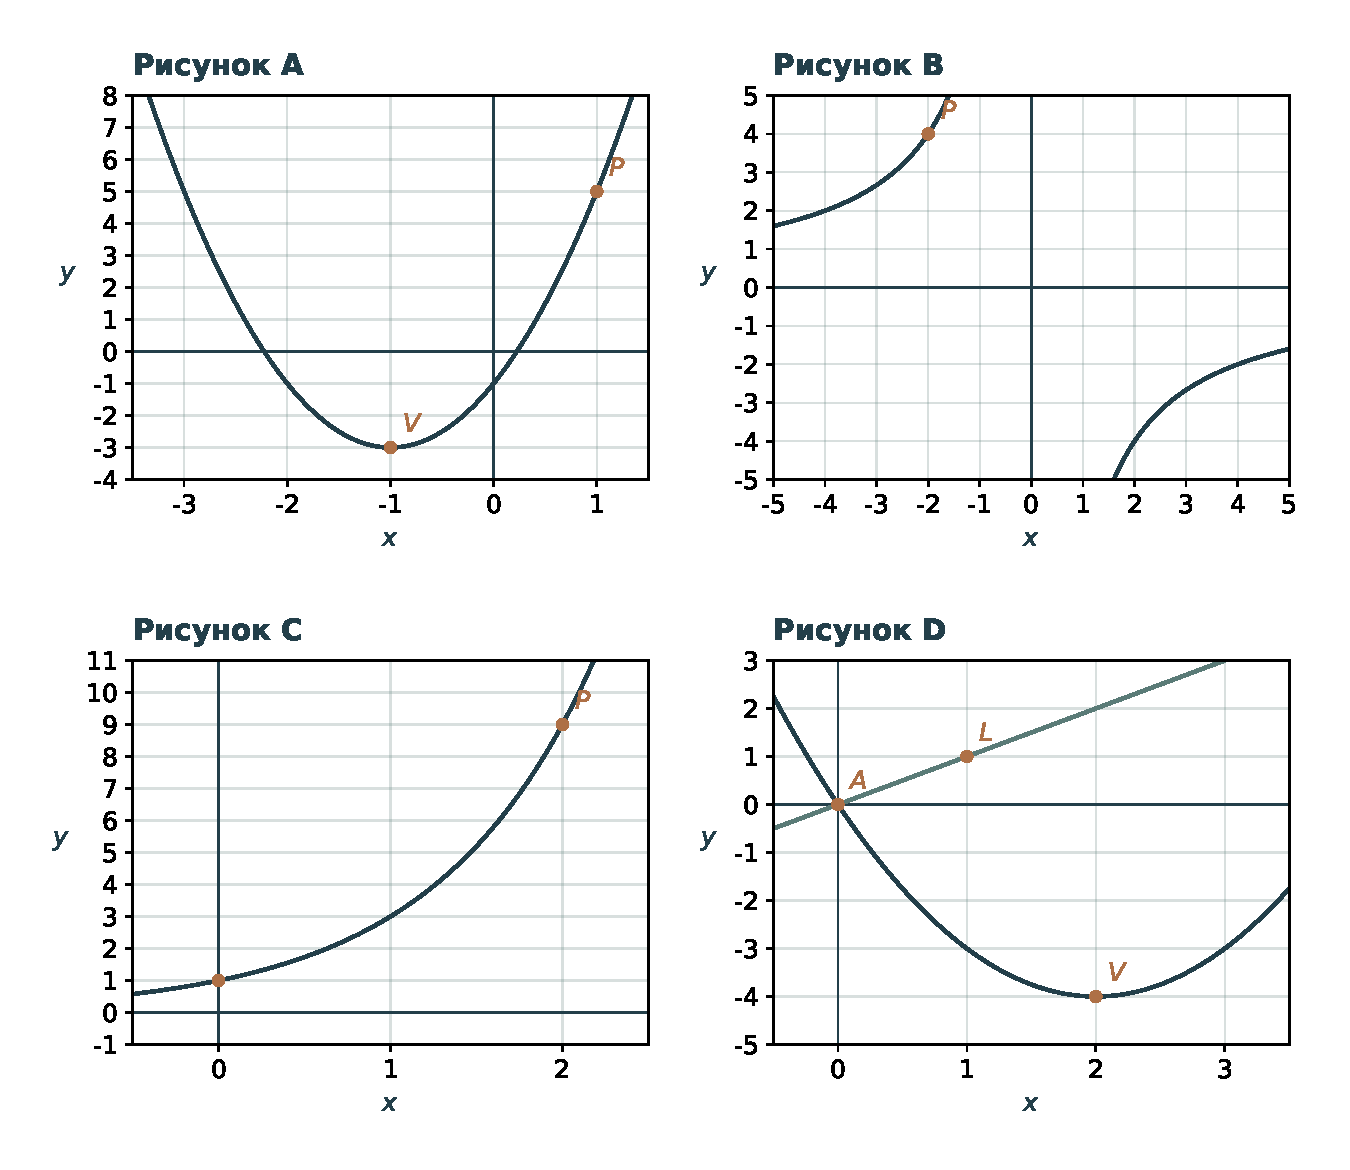
\includegraphics[width=\linewidth,height=135mm,keepaspectratio]{images/review-ege-functions.pdf}\end{center}
\par\addvspace{2pt}\begin{lrbox}{\CatFlowBox}\begin{minipage}[t]{\linewidth}
\setlength{\parskip}{2pt}\setlength{\columnsep}{4.5mm}\setlength{\intextsep}{0pt}
\begin{wrapfigure}[13]{r}{54mm}

\includegraphics[width=54mm,height=58mm,keepaspectratio]{images/unique/art-281.png}
\label{catflow:281}
\end{wrapfigure}
Чтение диаграммы начинается с того, какая величина отложена по каждой оси и в каких единицах она измеряется. Нулевой уровень, отрицательная высота и отсутствие столбца имеют разные значения. При сравнении двух моментов надо различать изменение на несколько единиц и изменение в несколько раз. Вопрос о первом подходящем месяце требует проверить порядок месяцев, а не только наибольший столбец. Если график соединяет отмеченные точки, точный ответ по изображению надёжнее извлекать в отмеченных узлах; поведение между ними должно быть задано отдельно. Для физической зависимости название оси также указывает, какая величина изменяется, а какая определяется по графику.
\par\WFclear\end{minipage}\end{lrbox}%
\ifdim\dimexpr\ht\CatFlowBox+\dp\CatFlowBox\relax<61mm\dp\CatFlowBox=\dimexpr61mm-\ht\CatFlowBox\relax\fi%
\noindent\usebox{\CatFlowBox}\par\addvspace{2pt}
\relax
\section{Данные на диаграмме: уровень, знак и первое совпадение}
У измерительного графика сначала читают подписи осей и цену деления. Вопрос «впервые» требует пройти данные слева направо, а вопрос «сколько раз» — посчитать все подходящие значения. Строгое сравнение с порогом отличается от нестрогого: столбец ровно на уровне порога в первом случае не подходит. Для отрицательных значений учитывают положение относительно нуля, а не высоту нарисованного прямоугольника без знака.
\begin{center}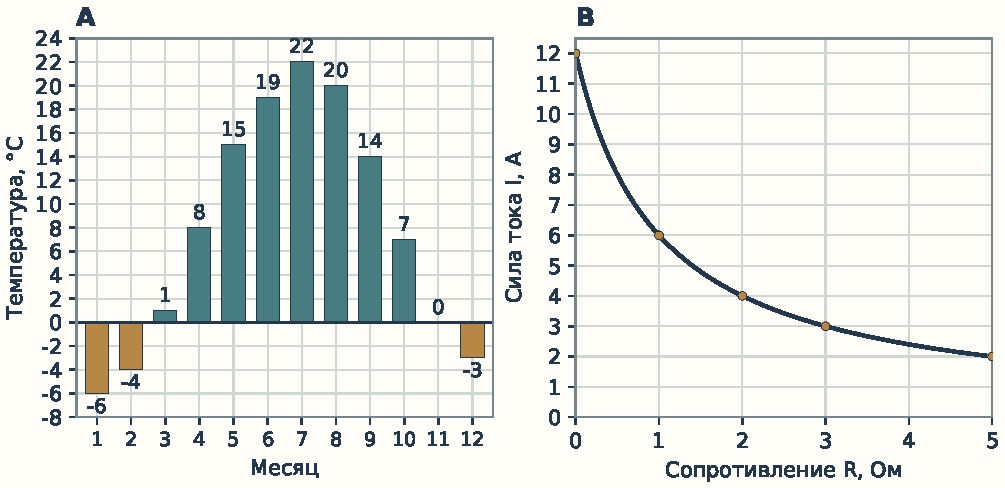
\includegraphics[width=\linewidth,height=78mm,keepaspectratio]{images/review-ege-data-reading.pdf}\end{center}
\begin{example}[Один рисунок, разные вопросы]\label{ex:review-ege-last-data}
На панели A средняя температура выше \(18^\circ\mathrm C\) в месяцах \(6,7,8\), всего три месяца. Отрицательные значения в месяцах \(1,2,12\), тоже три; нулевую температуру месяца \(11\) отрицательной не считают. Впервые ровно \(15^\circ\mathrm C\) наблюдается в месяце \(5\). Здесь сравниваются отдельные месячные значения: соединять вершины и искать промежуточный день условие не требует.
На панели B по горизонтали отложено сопротивление, по вертикали сила тока. При \(I=12\) А находим \(R=0\) Ом, при \(I=4\) А — \(R=2\) Ом. Сопротивление увеличилось на \(2\) Ом. Разность \(12-4\) относится к току и имеет другую единицу: она не отвечает на вопрос о сопротивлении.
\end{example}
\Needspace{7\baselineskip}\section*{Задачи}
\begingroup\setlength{\parskip}{1pt}
\noindent\begin{minipage}[t]{\linewidth}\textbf{21.1.} Найди область определения \(\dfrac{\sqrt{4-x^2}}{x-1}\).\par\end{minipage}\par
\noindent\begin{minipage}[t]{\linewidth}\textbf{21.2.} Построй \(y=|x-2|-1\). Найди вершину, нули и область значений.\par\end{minipage}\par
\noindent\begin{minipage}[t]{\linewidth}\textbf{21.3.} Как точка \((2;3)\) графика \(f\) переходит на график \(y=-2f(3(x-1))+4\)?\par\end{minipage}\par
\noindent\begin{minipage}[t]{\linewidth}\textbf{21.4.} Построй \(y=|x^2-4|\) и найди все решения \(y=3\).\par\end{minipage}\par
\noindent\begin{minipage}[t]{\linewidth}\textbf{21.5.} Построй \(y=(|x|-1)^2\). Найди нули и наименьшее значение.\par\end{minipage}\par
\par\addvspace{2pt}\begin{lrbox}{\CatFlowBox}\begin{minipage}[t]{\linewidth}
\setlength{\parskip}{2pt}\setlength{\columnsep}{4.5mm}\setlength{\intextsep}{0pt}
\begin{wrapfigure}[9]{r}{54mm}
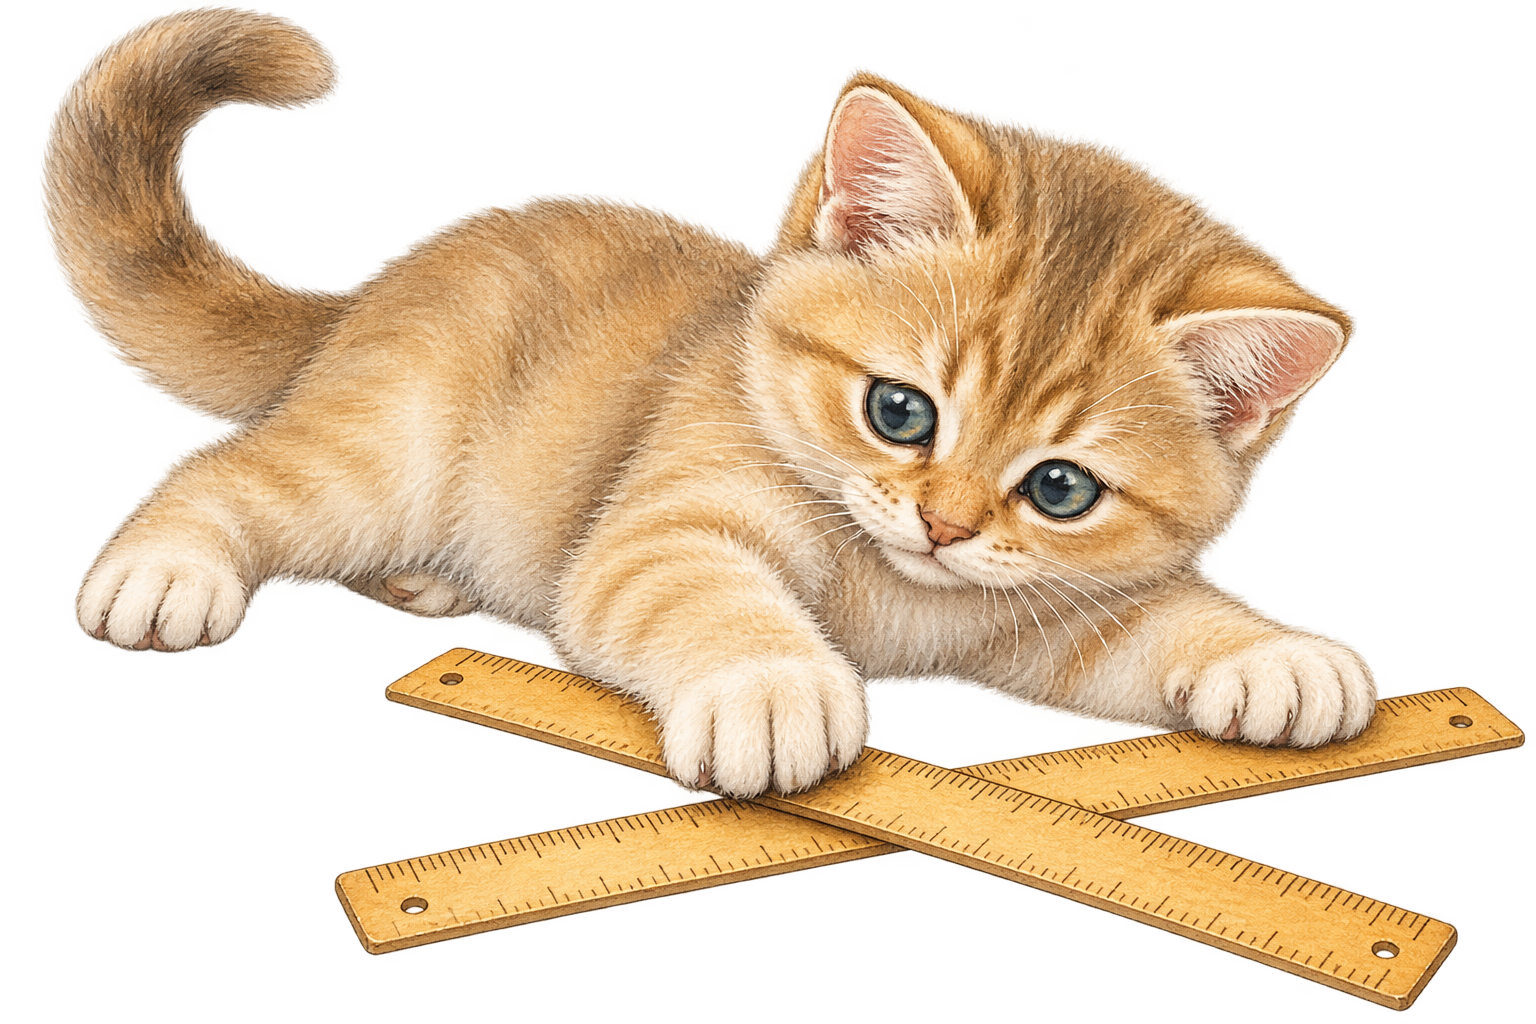
\includegraphics[width=54mm,height=58mm,keepaspectratio]{images/unique/art-216.png}
\label{catflow:216}
\end{wrapfigure}
\textbf{21.6.} Найди вершину, нули и промежутки знака \(x^2-6x+5\).\par

\textbf{21.7.} Найди минимум и максимум \((x-3)^2+1\) на \([0;2]\).\par

\textbf{21.8.} Найди минимум и максимум \(-x^2+4x\) на \([-1;3]\).\par

\textbf{21.9.} Преобразуй \(\dfrac{2x+3}{x-1}\) и укажи асимптоты.\par
\par\WFclear\end{minipage}\end{lrbox}%
\ifdim\dimexpr\ht\CatFlowBox+\dp\CatFlowBox\relax<58mm\dp\CatFlowBox=\dimexpr58mm-\ht\CatFlowBox\relax\fi%
\noindent\usebox{\CatFlowBox}\par\addvspace{2pt}

\noindent\begin{minipage}[t]{\linewidth}\textbf{21.10.} Опиши график \(\dfrac{x^2-9}{x-3}\) с учётом области определения.\par\end{minipage}\par
\noindent\begin{minipage}[t]{\linewidth}\textbf{21.11.} Является ли \(f(x)=x\), заданная только на \([0;1]\), нечётной?\par\end{minipage}\par
\noindent\begin{minipage}[t]{\linewidth}\textbf{21.12.} Найди наименьший положительный период \(\sin(3x)\).\par\end{minipage}\par
\noindent\begin{minipage}[t]{\linewidth}\textbf{21.13.} Для \(f(x)=2x+1\) при \(x<1\), \(f(x)=x^2+2\) при \(x\ge1\) найди \(f(0),f(1),f(2)\).\par\end{minipage}\par
\noindent\begin{minipage}[t]{\linewidth}\textbf{21.14.} Для функции из предыдущей задачи реши \(f(x)=6\).\par\end{minipage}\par
\noindent\begin{minipage}[t]{\linewidth}\textbf{21.15.} Найди область значений \(\dfrac1{x-2}+3\).\par\end{minipage}\par
\noindent\begin{minipage}[t]{\linewidth}\textbf{21.16.} Покажи, что \(\dfrac{1}{x}\) не является строго убывающей на всём множестве \(\mathbb R\setminus\{0\}\).\par\end{minipage}\par
\noindent\begin{minipage}[t]{\linewidth}\textbf{21.17.} Найди наклонную асимптоту \(\dfrac{x^2+2x+3}{x+1}\).\par\end{minipage}\par
\noindent\begin{minipage}[t]{\linewidth}\textbf{21.18.} Классифицируй поведение при \(x=1\) у \(\dfrac{x^2-1}{x-1}\) и \(\dfrac1{x-1}\).\par\end{minipage}\par
\noindent\begin{minipage}[t]{\linewidth}\textbf{21.19.} У \(f(x)=0\) при \(x<0\) и \(f(x)=1\) при \(x\ge0\) есть ли скачок в нуле? Каково значение в нуле?\par\end{minipage}\par
\noindent\begin{minipage}[t]{\linewidth}\textbf{21.20.} Найди число решений \(|x-1|=2-x\).\par\end{minipage}\par
\noindent\begin{minipage}[t]{\linewidth}\textbf{21.21.}\starmark{} Докажи преобразование точек для \(g(x)=af(b(x-h))+k\).\par\end{minipage}\par
\noindent\begin{minipage}[t]{\linewidth}\textbf{21.22.}\starmark{} Докажи, что \(f(x)+f(-x)\) чётна, а \(f(x)-f(-x)\) нечётна на общей симметричной области.\par\end{minipage}\par
\noindent\begin{minipage}[t]{\linewidth}\textbf{21.23.}\starmark{} Покажи, что график может пересекать горизонтальную асимптоту на примере \(f(x)=\dfrac{\sin x}x\), \(x\ne0\).\par\end{minipage}\par
\noindent\begin{minipage}[t]{\linewidth}\textbf{21.24.} Для \(f(x)=x\) на \((0;1)\) найди точные грани и выясни, достигаются ли они.\par\end{minipage}\par
\noindent\begin{minipage}[t]{\linewidth}\textbf{21.25.} Число решений \(x^2=c\) определи для всех действительных \(c\) по графику и алгебраически.\par\end{minipage}\par
\noindent\begin{minipage}[t]{\linewidth}\textbf{21.26.}\starmark{} Докажи, что строго монотонная функция на промежутке принимает каждое значение не более одного раза.\par\end{minipage}\par
\noindent\begin{minipage}[t]{\linewidth}\textbf{21.27.} На панели A изображена квадратичная функция. По отмеченным вершине \(V\) и точке \(P\) восстанови формулу, найди \(f(2)\) и оба нуля.\par\end{minipage}\par
\noindent\begin{minipage}[t]{\linewidth}\textbf{21.28.} На панели B показана функция \(f(x)=\dfrac{k}{x}\). Найди \(k\) и \(f(4)\) по отмеченной точке.\par\end{minipage}\par
\noindent\begin{minipage}[t]{\linewidth}\textbf{21.29.} На панели C изображена функция \(f(x)=a^x\), где \(a>0,a\ne1\). Найди основание \(a\) и \(f(-1)\). Почему одна точка \((0,1)\) не решила бы задачу?\par\end{minipage}\par
\noindent\begin{minipage}[t]{\linewidth}\textbf{21.30.}\starmark{} На панели D парабола и прямая пересекаются в отмеченной точке \(A\). По вершине параболы и точкам на прямой найди вторую общую точку, которая не помещается в показанном окне.\par\end{minipage}\par
\noindent\begin{minipage}[t]{\linewidth}\textbf{21.31.} По панели A найди: число месяцев с температурой не ниже \(19^\circ\mathrm C\); число месяцев со строго положительной температурой; первый месяц с температурой ровно \(0^\circ\mathrm C\).\par\end{minipage}\par
\noindent\begin{minipage}[t]{\linewidth}\textbf{21.32.} По панели B определи, на сколько омов изменилось сопротивление, когда сила тока уменьшилась с \(6\) до \(3\) А. Во сколько раз за это время изменилось сопротивление?\par\end{minipage}\par
\endgroup
